\documentclass[a4paper]{report}
\title{Using fNIRS to Detect Mental Workload and Emotional Valence in web form filling task}
\date{2015-09-18}
\author{Kristiyan Lukanov}
\usepackage{graphicx}
\usepackage{amsmath}
\renewcommand{\bibname}{References}
\begin{document}
	\pagenumbering{gobble}
	\maketitle
	\newpage
	\pagenumbering{arabic}
	
	\section*{Acknowledgements}
	blagodarq na toq i onq iuawhdauiwdaw joaiw joiakj aoif oiak opaekgpo kaeoikae 
	\newpage
	
	\section*{Abstract}
	taka i taka  oijga geriugj eurgjergijeigire eg jg eogpergkeprkgoe kpokepokgekgkegpokegpokepgkegk tgea tgwe gwe ghwgwhgrjtujdty
	\newpage
	\tableofcontents
	\newpage
	
	\chapter{Introduction}
	%The whole thesis should be third person past tense. Participants were asked to read and sign
	- Start with the problem
	
	Users often has to fill web pages containing more than 10 forms, like registering for a web site, posting classified ad, or sending online insurance claim. Sometimes this is really important, like filling insurance claim forms. People often dislike the fact that they should fill a long form and that makes the claim process difficult. That is why we are interested in measuring the mental workload in this type of tasks
	
	we want to if new web form designs will make the task easier
	
	
	Importance of those forms(how they should be accurate and unaiding)
	 However this often encountered task in our daily lives is not well researched in the field of cognitive science.	
	
	 -it is important measure, especially for critical tasks such as, aircraft controller, where operator with workload overload could cause accidents and cost human lifes.
	
	With the advance of technology, brain imaging techniques have emerged, like MRI, EEG, and fNIRS which were initially, used for medical research and purposes. In recent years the popularity of these brain imaging techniques has risen in the HCI field because of their ability to image brain data.
	
	videos shown are aversive stimuly(ili otbluskva6ti stimuli, ne e sigurno da se proveri) . 
	
	The studies using brain imaging were limited because they were presenting emotional cues, but in this study we check whether we can elucidate laterized emotions giving subjected emotional cue-less web interface. hich will be very useful in HCI area
	\section{Purpose of study}
		The purpose of the study is to find whether fNIRS can be useful for interface evaluations in HCI field. Also, we aim to find the most efficient layout for entering information on an web interface that has more than 10 forms , as this process is often encountered during daily web surfing, for example, when user registers to a new web site, or enter information for financial institutions, like insurance companies and banks.
	\section{Research questions}
		Can we measure mental workload with fnirs?
		- Could we detect emotional valence with fnirs?
		- Which of the three layouts is has the least mental workload and users preference?
		- Could we detect emotional valence, from web interface that has no emotional cues. This can very useful in HCI evaluations.
	\section{Industry partner}
		This work has been motivated by the need of entity partner funding my masters course. The industry partner has a insurance CRM software, and the aim of the study is to provide insights in the web form filling process by testing the layout of the web pages.
		
	\section{Structure of the thesis}
		In the next chapter we will first review the background literature behind usability and web forms, mental workload and working memory, Brain sensing techniques, Emotion processing. In chapter 3 we will describe the User study sectionexperiment done in the . And finally we will discuss the results from the experiment and propose a conclusion.
\chapter{Literature review}
	The aim of Human Computer Interaction(HCI) field is to propose methodologies for evaluation and improvement of computer interfaces because they are often complex and hard to understand for the average users. The HCI literature divides two main classes of evaluation methods: quantitative and qualitative. On the one hand, quantitative methods provide objective data like, task completion time, number of errors or other numerical data. On the other hand, qualitative methods gave subjective data in the form of user opinions, observed behaviour and etc. Moreover, Nielsen\cite{nielsen1994measuring} have found that user preferences do correlate with user performance, thus we can rely solely on user preferences, however this is not always the case. Consequently, Nielsen and Levy \cite{nielsen1994measuring} advise researchers to use combination of subjective and objective data, in order to identify bias and provide richer information. Hence, we have decided to employ user trials(qualitative data) combined with psychophysiological measurements(quantitative data). In addition, functional near infrared spectroscopy (fNIRS), has been recently suggested as a promising method for HCI evaluations\cite{maior2015examining,pike2014measuring} because it can measure mental workload\cite{maior2014continuous}.  Based on this, we decided to test the usefulness of fNIRS in HCI evaluation studies. We are concerned with desktop interfaces, or more specifically web interface. The domain chosen for the usability study is insurance software because the industry partner needs more information about the web form filling and design process. 
	
	evaluation of interfaces like, user trials, interviews, questionnaires, think aloud protocols and more. However, as the technology is advancing and new computer interfaces created, the need for more evaluation methods is increasing[]. In this study we are concerned with web interfaces because they are the most used ones.
	
	Overview of HCI evaluations, and quickly exclude large sections of it, so we are interested in usability of web forms. Interviews will tell us what users think about the interface. Usability assessments will tell us what use expert think about it. Observation will let you see the paviors of people while using web forms. Our research questions for this master thesis are to do with mental workload and short interviews will
	
	what is usability and human computer interaction - Sarah's slides
	what are the goals of usability and user experience -- user experience honey comb
	
	We prefer studies where we can combine subjective and objective data so that
		
	Evaluation methods - observations, user trials, interviews, questionnaires?
			
	Because of insufficiency of relevant literature on the web form filling and design we are going to examine general usability guidelines and recommendations as they are widely accepted by the Human Computer Interaction researchers. The two most popular usability heuristics are those of Nielsen\cite{nielsen1990heuristic}, and Shneidermann\cite{shneiderman1992designing}. They express similar suggestions, like, maintain consistency, provide feedback, support expert users, prevent and optimize error messages, provide help documentation, permit easy reversal of information, and minimize working memory load. Consequently, the design of the tested variants in the usability study in chapter 3 is informed by them. Also, because both heuristics advocate minimizing the load on working memory we consider that reducing it will provide better user experience.
	Performance measures
	%	What is usability - briefly
	%	Usability Evaluation methods
	%	- heuristics
	%	- observations
	%	- performance measures
	\section{Usability and Web form filling}	
			Web form filling is often encountered activity in daily surfing of web users, however, according to our knowledge, there is scarce of empirical research in the Human Computer Interaction(HCI) literature for this topic. First, a study by Wästlund\cite{Wastlund20081229} compared two web page layouts - one that all the text is in the same page, and one where the text is separated in four pages. Authors concluded that users experienced less workload with the divided web form(4 pages), compared to the single page web form. Second, two books specially written for web form filling design\cite{jarrett2009forms,wroblewski2008web} suggest splitting long web forms into several pages, in order to improve the process. Lastly, most of the research on web form filling and design is focused in optimizing the experience and accessibility for elderly population\cite{sayago2012selective,chadwick2003web,lines2006online,sayago2007some}.\\
			
		 
			
			To find the best variation researchers use performance metrics like, task completion time, number of errors made, quantity of information provided and more.
		
			
			at hand we will use the usability heuristics proposed by Norman\cite{nielsen1994usability,nielsen1990heuristic} and Shneiderman\cite{shneiderman1992designing}. Heuristic designed specially for web interfaces 2007. Gulf of evaluation and gulf of execution(maybe).  - two books on web forms\\
			cite some general recommendations for web forms and design
			-most of the usability relies on descriptive recommendations.
			Because usability of certain interface depends on the context, user differences, and that there is not perfect solution to a interface problem, and designers often have to make tradeoffs, we will rely on cognitive science in order, to predict which layout is more appropriate
			
			A couple of studies suggest that the longer it takes for a task(short or long term) to be completed the more the perceived frustration the users experience increases\cite{mendoza2005usability,bessiere2004social}.
		
	\section{Working Memory and Mental Workload}
		The concept of mental workload (MW) is intuitive in nature and it represents how busy an operator is when performing a certain task. The concept has been referred in the literature with many terms, like cognitive load, stress, strain, and arousal. The aim is to Many definitions has been proposed by many authors, however researchers are still unable to find a consensus on the term[Linton et al 1989]. Wickens\cite{wickens2008multiple} defines it as "The demand imposed by tasks on the human's limited resources, whether considered single or multiple". Depending on the studied task at hand, knowing workload experienced by different design variations will help choose the one that generates desired operator performance. Also, in terms of operator experience of MW, Rouse et al classifies different factors like, fatigue, mood, individual differences, as person-specific workload\cite{rouse1993modeling}. Similarly, Norman and Bobrow classified operator performance on data-limited and resource-limited\cite{norman1975data}. They hypothesize that even if operator spends high amount of attentional resources, the task can have a bad representation that will degrade the performance. In contrast, resource-limited performance depends on how much attentional resources the task demands, and it can be considered that every real life task consists of combination of both. 
			\subsection{Working memory models}
			Rather than searching for definition researchers in cognitive science use models of working memory in order to understand cognition, predict and explain workload and performance. Furthermore, theories of working memory try to define the processes going into human mind, and explain concepts such as, attention, perception, long term memory, decision making, action selection, and execution\cite{wickens-1988,baddeley1974working,miller1956magical}. Most of those models are based on human as information processor approach \cite{broadbent1,broadbent2,neisser,wickens-1988}, which relates the processes of human mind with those of a computer processor. Also, the framework is based on the assumption that the human operator has a limited resource capacity[], and if the task demands more resources than the capacity of the operator, workload overload is observed. Moreover, the information from the environment or the task is processed by series of processing systems, like perception, attention, short-term memory, long-term memory. 
			In attempt to describe the web form filling task we can use the working memory model from Baddeley and Hitch \cite{baddeley1974working} which processes information in verbal and spatial form . It consists of a central executive, which is acts as an administration system which controls the information input and output of its slave systems. The visuo-spatial sketch pad is involved in holding visual information in spatial form like, objects and colours. The phonological loop stores verbal information, such as words and names. And the later proposed \cite{baddeley2000episodic} episodic buffer is responsible for the storage and retrieval of memories or events. Because the task of web form filling involves multiple cognitive processes like, visual search, speech synthesis, planning, memory retrieval, decision making, thus utilizing all slave systems of the model, we can label the web form filling process as one that involves complex cognition. 
				\begin{figure}[h]
					\centering
					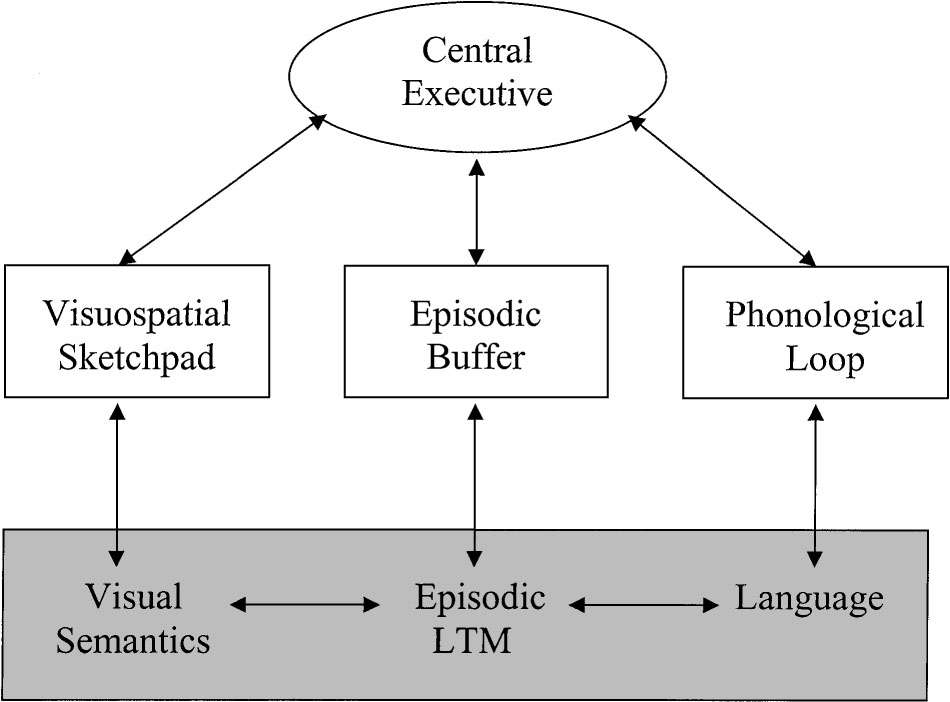
\includegraphics[width=0.5\linewidth]{baddeley-wm}
					\caption[Baddeley and Hitch Working memory model]{Working memory model by Baddeley and Hitch, displaying the 'slave systems' visuo-spatial sketch pad, episodic buffer and phonological loop, controlled by the central executive.}
					\label{fig:baddeley-wm}
				\end{figure}		
				

			We can also consider the multiple resources model by Wickens\cite{wickens2008multiple,wickens2002multiple} which is suited for predicting the workload of an operator performing multiple tasks at one time. The approach is based on four basic assumptions:\\

			1) in the stages of processing dimension, perceptual and cognitive tasks use different resources than response selection and execution;\\
			2) spatial activity uses different resources than verbal or linguistic activity;\\
			3) the modalities dimension, different resources are used for auditory and visual perception\\
			4) visual channels are divided on focal and ambient vision\\
			And the main argument of the theory is "to the extent that two tasks use different levels along each of the three dimensions, time-sharing will be better" \cite{wickens2008multiple}. The model provides an account on how different elements of the human information processor, like attention, perception, working memory, response selection and execution interact between each other. This theory is also based on evidence from cognitive neuroscience where we can see that different modalities have different locations in the human brain, like primary auditory cortex is involved with auditory perception[] and the visual perception is processed in the occupational lobe[].\\
							\begin{figure}[h]
								\centering
								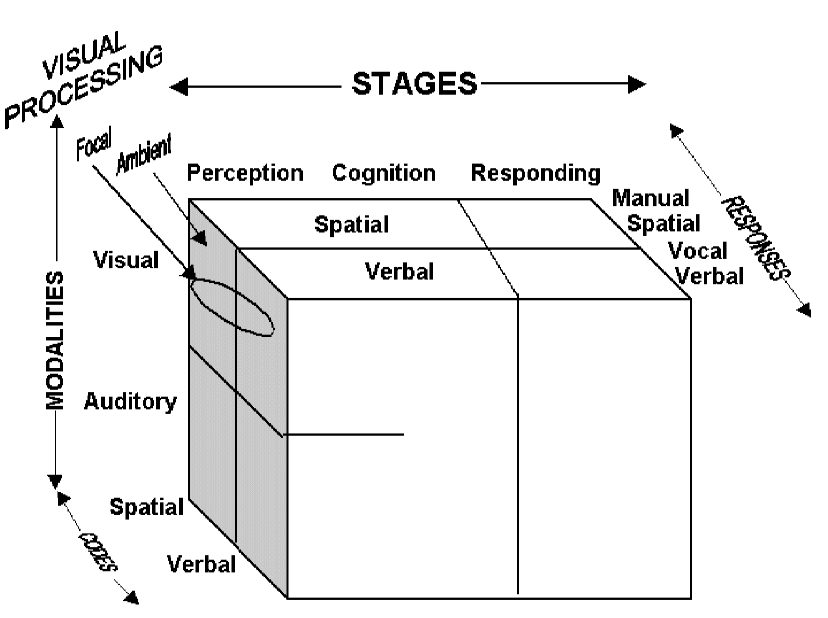
\includegraphics[width=0.7\linewidth]{mrt}
								\caption[Multiple resource theory by Wickens]{Wickens 4-D multiple resources model}
								\label{fig:mrt}
							\end{figure}
			However, mental workload can be influenced by the initial perception of the task at hand or the 'appraisal' of it. Similarly to MW appraisal is complex and multidimensional concept\cite{folkman1986dynamics,peacock1990stress} that is not well defined.
		
		
			\subsection{Measuring Mental Workload}
			The concept has been explained differently by different authors, and inferences made from various empirical measures which can be divided on primary, secondary, subjective and psychophysiological measures. There are also analytical techniques but we are not concerned with them in this dissertation.
				\subsubsection{Primary and secondary task mesures}
				Primary measures rely on operator performance to predict workload. However, a limitation of using primary measures alone is that an operator can spend high amount of effort but this may not be apparent from the performance\cite{wilson2015evaluation}. Consequently, primary task measures should be combined with other workload measures. An example performance measures are task completion time, number of errors, and response time. In our case we will use a combination of all but secondary task measures. Secondary task involves inclusion of a additional simple task to the primary one, which is done concurrently, if the primary task has low or moderate demand and the level of workload cannot be inferred only from the primary measure. It is used to detect when operators performance deteriorates and this is due to workload overload. However, as we are not going to use secondary measures, more explanation will provided for the other types of measurements.
				\subsubsection{Subjective measures}
				Subjective measures use rating scale and are based on operator opinion of their perceived workload during or after completion of task. They are preferred method for WL estimation because they are easy to administer, cheap, and with high face validity. They are classified as uni dimensional and multidimensional. They consist of single subjective scale of workload and multiple scales of types of workload, accordingly. From the unidimensional subjective measures the Cooper-Harper\cite{cooper1969use} is the most popular among ergonomists and cognitive researchers. However, it is designed for the aircraft domain, and therefore a modified cooper-Harper scale\cite{wierwille1983validated} was created for use in other domains. However, as mental workload is influenced by different environmental and personal factors\cite{rouse1993modeling}, therefore the concept of MW should be considered as multidimensional concept, in order to improve diagnosticity. Accordingly, multi-dimensional subjective scales should be used to better understand the aspects of MW. The most used scales are NASA-TLX\cite{nasatlx}, SWAT\cite{reid1988subjective} and Workload profile\cite{tsang1996diagnosticity}. NASA-TLX is based on rigorous laboratory research, and it includes 6 scales (mental, physical, temporal demand, experienced effort, frustration and performance) consisting of 20 intervals each and it is relatively easy to administer. In addition, a single measure of workload can be weighted, although it is not necessarily required because there is high correlation between weighted and unweighed results\cite{byers1988workload}. 
				The SWAT subjective scale is also widely used, however the process of implementation is laborious and more complex than the other subjective scales. The other popular scale is Workload profile(WP)\cite{tsang1996diagnosticity} scale which is basen on the Wickens multiple resources model, and asks questions about each of the four dimensions proposed by the theory. Hence, it is very useful when combined with multiple resource theory interpretation of the results. Finally, Longo et al. \cite{longo2012importance} compared the three measures mentioned above in a web browsing/searching task, and observed correlations in the results of the three measures claiming that they measure the same concept of mental workload.\\
				\subsubsection{Psychophysical measures}
				Psychophysical measures are used to give objective data about mental workload by not relying on subjective scales or performance measures . They can be obtained by recording cardiac activity, electrodermal activity, eye function or imaging the brain. These techniques detect the  change in the arousal from the autonomic nervous system level which can be inferred to as mental workload. However, different psychophysical measures capture different aspects mental workload\cite{cain2007review}, therefore consideration should be put in choosing the most appropriate measure for the given task. \\
				Mean heart rate(HR) and heart rate variability(HRV) are one of the most used techniques to infer arousal because it is relatively cheap and easy to administer. However, HR not always correlates to subjective measures of MW\cite{haapalainen2010psycho} and because of this HRV can be considered as more valid measure. Moreover, the beat to beat interval of the heart can be measured using different statistical approaches\cite{billman2011heart}, like, standard deviation from heart beat intervals. Measurements of eye activity, like blink rate, pupil diameter are also being found to correlate to MW. Furthermore, increase in pupil diameter is correlated to rise in arousal \cite{kahneman1973attention}, and Beatty claimed that it has high sensitivity \cite{beatty1982task} and it can be used to distinguish between data-limited and resource limited processing, which can make it very useful in the HCI field. However, incoming light at the eye can change the pupil diameter, which is a process unrelated to the task, thus influencing the measurements, therefore it is suitable for experiments in controlled environment. \\Finally, a number of brain imaging techniques are used to obtain measurements from the brain activity, including electroencephalography(EEG), functional near-infrared spectroscopy(fNIRS), functional magnetic resonance imaging(fMRI), however these will be discussed later in section "Brain sensing".
		
		 %and yielded similar results, suggesting they measure the same aspects of the web task. The author infers that only one mental workload measure is required. Because mental workload is influenced by a number of factors, and therefore it is multidimensional concept, NASA-TLX is chosen as subjective measure for the experiment.
		
 
		 %Lavie(2005,2010) Load theory says high perceptual load decreases attention to distractions, and low perceptual load increased them. High perceptual load is experienced when, for example, driving fast a car, or playing sports. Furthermore, because it involves a lot of perceptual capacity there is no spare capacity for the attention to perceive distractions. In this case, the task has a low perceptual load because it demands only to a visual stimuli to be percieved and processed rather than with audioty, o
	\section{Brain sensing}
		discuss the different brain imaging techniques, - MRI, EEG, fNIRS. Because fnirs is portable, n
			\subsubsection{PFC and arrousal and affect}
			The prefrontal Cortex is involved with higher cognitive functions and emotion processing.
			\subsubsection{Fnirs and mental workload}
			- PFC is involved in cognitive control(higher cognitive abilities) functions \cite{fawfa,dawda,dawwd}
			Highlight studies involving mental workload.
			More specifically,
			there is a positive correlation between the increase of oxygenated blood and the
			increase in cognitive WL- 
			-limitations
			has low temporal resolution
			\subsubsection{Galvanic skin and mental workload}
			Highlight studies involving mental workload.

	\section{Studies on Emotion}
			It has been suggested that processes involved with emotion processing are situated in the Prefrontal cortex (PFC) \\cite{rwa}
			-appraisal studies
			There are several anticipation studies
			We do not anticipate to detect any activation in the PFC or because [1,2,3] studies of anticipation of pain activated only the cingulate, insula and amygdala regeins which all are in vutre6nosta of the brain which the fNIRS device cannot detect.
			 Furthermore, one of the many proposed dimensions is 'anticipated effort'\cite{smith1985patterns} where the motivation for executing the task can be altered by the appraisal of the task. For example, if operator appraises the task as one that has to be invested high amount of effort, a challange emotion is associated. If the expected effort is moderate hope and interest should be experienced, and finally boredom is felt when the anticipated effort is low. 
			
			
	\section{fNIRS and Emotional Valence}
		It is still not proven that activation in the left hemisphere is responsible for the processing of positive emotion.
		gender differences, 
		left-right handedness
		1. Emotional induction - when pictures or videos or other method is used to trigger certain kind of emotion
		Emotional regulation
		- apprisal
		- reapprisal - kogato si spomnime i preocenim dadena emociq (cognitively reexamine the meaning of emotional events)
		- anticipation of expected outcomes 
		- In this study we have combined "hot" emotional control  with cold control of attention and memory, as suggested by Kevin N. Ochsner and James Gross \cite{the-cognitive-control-of-emotion}
		-Richard Davidson first a comprehensive research in the topic cortical assymetry
	\section{Summary}
		Because not many researchers[] do not take in consideration the emotional state(positive or negative) which can be related to aproach and avoid motivation during task execution, and how it influences the performance of the operator and perceived workload, we have combined multidimensional subjective scale (NASA-TLX) with emotional valence scale (SAM). By combining the these subjective measures and comparing them the objective measure of mean Hbo from the fNIRS device we expect to gain better understanding of the operator performance during the web form filling task.
		Arrousal should correlate with skin conductance.
		We are aiming to reduce to imposed load by the task by minimizing the visual search(condition3) and aiding the episodical memory by placing a description in the beginning of the form.
\chapter{User study}
	\section{Hypothesis and expectations}
	Based on the literature review we state the following hypothesis:\\
	1) There is statistical difference between the three web forms\\
	2) Subjective data from NASA-TLX correlates to objective data from the fNIRS\\
	3) The difference in left and right hemisphere activations correlate to subjective SAM scale of emotional valence\\	
	\section{Method}
	Describe why I have used the following methods, including the perceived benefits of your approach\cite{preferences-study}.
		\subsection{Participants}
		\subsection{Apparatus}
			\subsubsection{Laptop computer}
			The experiment was executed on 15" laptop, HP probook 450 with screen resolution 1366x768. The participant was presented with a screen with links to the three different videos and web forms. They were instructed by the researcher to manually start certain condition or video. 
			\subsubsection{fNIRS}
			Picture of fNIRS\\
			730nm and 850nm wavelengths will be collected for each voxel, eliminating the ambient light. . However, if the data acquisition computer does not have enough bandwidth,
			one or more of the quadrants can be disabled to maintain 2Hz sampling rate. 
			\subsubsection{Empatica}
			Picture of Empatica E3\\
			Before attaching the Epatica E3 the skin was treated with alcohol for better conductivity.
        \subsection{Materials}
			\subsubsection{NASA TLX}
			\subsubsection{SAM}
			\subsubsection{Web forms}
			\subsubsection{Video capture}
		\subsection{Design}
		The study used repeated measures within subjects designThe three variations of videos and the web forms were counterbalanced, in order to
		Performance measure - characters written in the description field
		\subsection{Procedure}
		First, participants were asked to read and sign information sheet and consent forms. Second, the Empatica E3 and fNIRS devices were cleaned then equipped and started. Third, participants were briefed about the procedure of the experiment, and it was explained how to fill the subjective scales. Also, because of ethical considerations that the participant should not enter personal data in the web form, a fake personal credentials were provided, that she should fill in the web forms. Fourth, after the video capture, fnirs and empatica devices started recording data, participants were asked to open one of the three videos, depending on the counterbalancing table. After the video was finished, participants fill SAM subjective scale. Fifth, there was approximately 2 minute waiting period so that participant's memory is not fresh before she was asked to open one of the three web forms, again depending on the order from the counterbalancing table. Finally, after participant has completed the web form, the SAM and then the NASA-TLX scales are given to be completed, accordingly. This process was repeated three times, following the within subjects experimental design.
		Before each experiment, the clocks between the two computers (the one that was obtaining the information and one that participant worked on) were synchronized. Also, timestamps using the Cobi Studio software manual markers were created in the beginning and end of each condition and video. 
		\subsection{Data Analysis}
		The fNIRS data was analyzed with NIRS-SPM\cite{ye2009nirs}		
			\subsubsection{Signal acquisition}
			What is the task - it is not mental aritmetic, or mental imagery, it is complex web form filling task.
			\subsubsection{Preprocessing}
			Instrument noise was reduced by placing a hat over the fNIRS headband, in order to block external light.
			First, low-pass filter with cut off frequencies of 0.1 Hz, was used in order to remove physiological noise, like heartbeat and blood flow movement that is not associated with brain activity or Mayer waves.
			Then, the NIRS signal was processed with modified Beer-Lambert law\cite{cope1988system}, in order to calculate oxygenated, and deoxygenated hemoglobin values.
			Finally, to remove motion artefacts, the correlation based signal improvement(CBSI)\cite{cui2010functional} method was applied to the data.
			\subsubsection{Feature Extraction/selection}
			After data preprocessing we should choose what features we will use to evaluate our data - mean values of oxy-Hb, mean values of oxy-Hb for all channels, skewness, variance
	\section{Results}
		\subsection{Mental Workload}
			\subsubsection{fNIRS data}	
			A one-way repeated measures ANOVA was conducted to determine whether there was a statistically significant difference in mean Hbo values between the three web forms. The assumption of sphericity was met, as assessed by Mauchly's test of sphericity, $X^{2}(2) = 0.195, p = 0.907$. There was no significant statistical difference in the mean Hbo between the 3 web forms  $F(2,20)=3.400, p<.054,$ partial $\eta^{2}=.254$ with mean Hbo decreasing from 0.2377 (SD = 1.19) in index3 to -0.1166 (SD = 0.82) and -0.117 (SD = 1) for index2 and index1 respectfully. 	
				\begin{figure}[h]
					\centering
					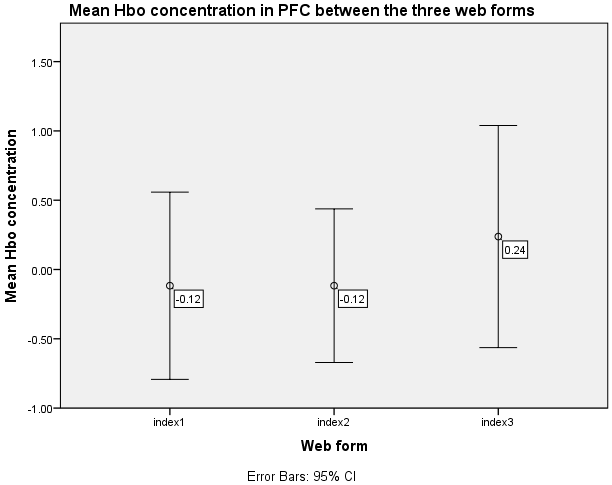
\includegraphics[width=0.7\linewidth]{mean-hbo-index123}
					\caption[Mean oxygenated hemoglobin between the three web forms]{}
					\label{fig:mean-hbo-index123}
				\end{figure}	
			No statistical significance was found when comparing the means of Hbr between the three conditions $F(2,20)=2.044, p<.156,$ partial $\eta^{2}=.170$ where index2 had the highest Hbr mean 0.05 (SD = 0.85), index1 with -0.07 (SD = 0.96) and index3 with the lowest Hbr mean -0.36 (SD = 1.43). and Hbt $F(2,20)=0.685, p<.516,$ partial $\eta^{2}=.064$.
			There were no correlation between Hbo and other measures.
			\subsubsection{NASA-TLX}
			There was no statistical significance between each of the NASA-TLX scales, including the total score as assessed by one way repeated measures ANOVA.
			There was a moderate positive correlation between mental demand scales and task completion times between the three conditions  $r(18)=0.487, p=0.030,  r(18)=0.484, p=0.030,  r(18)=0.638, p=0.002$. Also, mental demand scales had a moderate positive correlation with the total NASA-TLX between the three conditions $r(18)=0.652, p=0.002,  r(18)=0.738, p=0.0005,  r(18)=0.741, p=0.0005$
			\begin{figure}[h]
				\centering
				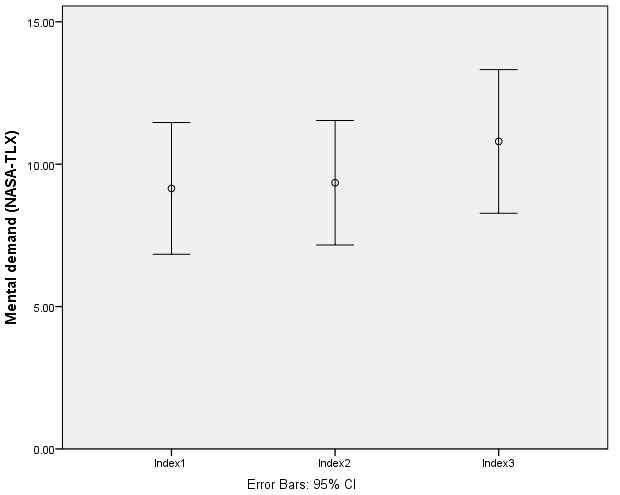
\includegraphics[width=0.6\linewidth]{mental-demand-graph}
				\caption{}
				\label{fig:mental-demand-graph}
			\end{figure}
			\subsubsection{SAM - subjective arousal scale}
			No statistical significance was found when comparing the means of SAM arousal scale between the three conditions $F(2,38)=2.462, p<0.099,$ partial $\eta^{2}=.115$ using one way repeated measures ANOVA. However, after running post hoc test without adjustments(LSD) a statistically significant difference was found between index1 and index3 $p=0.049$.
			Also, the time to complete index1 and index2 positively correlated to perceived arrousal for index 1 and index2:$r(18)=0.551, p=0.012,$ and $r(18)=0.473, p=0.035,$. However time to complete index3 does not correlate to perceived arrousal of index3 $r(18)=0.269, p=0.252$
			
		\subsection{Emotional Valence}
			\subsubsection{fNIRS differences}
				WEB FORMS\\
				 There was no statistical significance as assessed by one way repeated measures ANOVA between the three conditions for Hbo valence differences: $F(2,20)=0.392, p<0.681,$ partial $\eta^{2}=.038$ , Hbr valence differences: $F(2,20)=0.418, p<0.664,$ partial $\eta^{2}=.040$ and Hbt valence differences: $F(2,20)=0.302, p<0.743,$ partial $\eta^{2}=.029$.\\
				 Also, there was strong positive correlation between temporal NASA-TLX scale of index1 and the Hbo valence differences of index1 $r(9)=0.766, p=0.006$, however, there was no correlation found between index2: $r(9)=0.581, p=0.061$ and index3: $r(9)=0.218, p=0.519$.\\
				VIDEOS\\
				A one-way repeated measures ANOVA was conducted to determine whether there was a statistically significant difference in Hbo, Hbr and Hbt valence differences between the three videos. There was no significant statistical difference in the mean Hbo valence difference between the 3 videos $F(2,20)=0.051, p<0.951,$ partial $\eta^{2}=.005$, the mean Hbr valence difference: $F(2,20)=0.062, p<0.940,$ partial $\eta^{2}=.006$ and the mean Hbt valence difference: $F(2,20)=0.522, p<0.601,$ partial $\eta^{2}=.050$.
				There was no correlation found between Hbo valence differences and SAM emotional valence subjective scale for the three videos $r(9)=-0.490, p=0.126$; $r(9)=0.095, p=0.781$; $r(9)=0.496, p=0.121$. 
			\subsubsection{SAM emotional valence}
			WEB FORMS\\
			A one-way repeated measures ANOVA was conducted to determine whether there was a statistically significant difference in SAM emotional valence scale values between the three web forms. The assumption of sphericity was met, as assessed by Mauchly's test of sphericity, $X^{2}(2) = 0.446, p = 0.800$. There was no significant statistical difference in the SAM emotional valence scale between the 3 web forms  $F(2,38)=2.803, p<.073,$ partial $\eta^{2}=.129$ with mean SAM emotional valence increasing from 3.1$\pm$0.97 in index1 to 3.4$\pm$0.99 and 3.7$\pm$0.98 for index2 and index3 respectfully.
			VIDEOS
			There was no statistical significance as assessed by one way repeated measures ANOVA between the three videos for SAM emotional valence: $F(2,38)=0.792, p<0.460,$ partial $\eta^{2}=.040$
		\subsection{User performance and preferences}
		A one-way repeated measures ANOVA was conducted to determine whether there was a statistically significant difference in time to complete between the three web forms. There was no significant statistical difference in time to complete between the 3 web forms  $F(2,38)=0.556, p<.578,$ partial $\eta^{2}=.028$. 
		Also, the time to complete index2 and index3 had a strong positive correlation with perceived effort(NASA-TLX) for index2 and index3: $r(18)=0.702, p=0.016,$ and $r(18)=0.634, p=0.036,$. However, time to complete index1 does not correlate to perceived effort of index1 $r(18)=0.216, p=0.524$

\chapter{Discussion}
	What was the purpose of the study, and then interpretation of the results
		\subsection{Implications for Design}
		\subsection{Disadvantages of the study}
		The study tries to simulate real conditions, and therefore lacks ecological validity because users wait approximately 2 minutes after they have watched the video to start filling the web form. This way they still hold some of the information in their working memory and the study is trying to simulate long term memory recall.
		\subsection{Future work}
	\section{Conclusion}
	In summary, the mental workload is lower for this....


	\addcontentsline{toc}{chapter}{References}
	\bibliographystyle{plain}
	\bibliography{exmplref}
	\addcontentsline{toc}{chapter}{Appendix}
\chapter*{Appendix}
\end{document}